\section{Progettazione concettuale}

\subsection{Analisi delle entità}

%Marina
\begin{center}
    \begin{tabularx}{\textwidth}{|l|l|l|X|}
        \hline
        \rowcolor{gray!30}
        \multicolumn{4}{|c|}{\textbf{Marina}}\\
        \hline
        CoordinateGeografiche & VARCHAR & Identifica univocamente la posizione del marina & Chiave \\
        \hline
        Nome & VARCHAR & \multicolumn{2}{l|}{il nome del marina} \\
        \hline
        QtMoli & INTEGER & \multicolumn{2}{l|}{Quantità di moli presenti nel marina} \\
        \hline
    \end{tabularx}
\end{center}

%Imbarcazione
\begin{center}
    \begin{tabularx}{\textwidth}{|l|l|l|X|}
        \hline
        \rowcolor{gray!30}
        \multicolumn{4}{|c|}{\textbf{Imbarcazione}}\\
        \hline
        Coordinate internazionale & VARCHAR & Identifica univocamente un'imbarcazione nel mondo & Chiave \\
        \hline
        Nome & VARCHAR & \multicolumn{2}{l|}{Il nome dell'imbarcazione} \\
        \hline
        QtPostiLetto & INTEGER & \multicolumn{2}{l|}{La quantità di posti letto dell'imbarcazione} \\
        \hline
        Capitano & VARCHAR & \multicolumn{2}{l|}{Il nome del capitano} \\
        \hline
        Bandiera & VARCHAR & \multicolumn{2}{l|}{Nome dello stato di cui batte bandiera l'imbarcazione} \\
        \hline
        Dimensioni & VARCHAR & \multicolumn{2}{l|}{Attributo composto: Pescaggio, Larghezza, Lunghezza} \\
        \hline
    \end{tabularx}
\end{center}

%Molo
\begin{center}
    \begin{tabularx}{\textwidth}{|l|l|X|}
        \hline
        \rowcolor{gray!30}
        \multicolumn{3}{|c|}{\textbf{Molo}}\\
        \hline
        Occupato & BOOLEAN & Lo stato di occupazione del molo\\
        \hline
        Dimensioni & VARCHAR & Attributo composto: Pescaggio, Larghezza, Lunghezza \\
        \hline
    \end{tabularx}
\end{center}

%Persona
\begin{center}
    \begin{tabularx}{\textwidth}{|l|l|l|X|}
        \hline
        \rowcolor{gray!30}
        \multicolumn{4}{|c|}{\textbf{Persona}}\\
        \hline
        CF & VARCHAR & Identifica univocamente una persona & Chiave \\
        \hline
        Nome & VARCHAR & \multicolumn{2}{l|}{Il nome della persona} \\
        \hline
        Cognome & VARCHAR & \multicolumn{2}{l|}{Il cognome della persona} \\
        \hline
        DataNascita & DATE & \multicolumn{2}{l|}{La data di nascita della persona} \\
        \hline
        Contatto & VARCHAR & \multicolumn{2}{l|}{I contatti della persona(multi-valore)} \\
        \hline
    \end{tabularx}
\end{center}

%Cliente
\begin{center}
    \begin{tabularx}{\textwidth}{|l|l|X|}
        \hline
        \rowcolor{gray!30}
        \multicolumn{3}{|c|}{\textbf{Cliente}}\\
        \hline
        Cittadinanza & VARCHAR & Lo stato di cui il cliente è cittadino\\
        \hline
        Residenza & VARCHAR & Lo stato in cui il cliente è residente \\
        \hline
    \end{tabularx}
\end{center}

%Cliente occasionale
\begin{center}
    \begin{tabularx}{\textwidth}{|l|l|X|}
        \hline
        \rowcolor{gray!30}
        \multicolumn{3}{|c|}{\textbf{Cliente occasionale}}\\
        \hline
        MarinaVisitati & INTEGER & Il numero di marina che il cliente ha visitato \\
        \hline
    \end{tabularx}
\end{center}

%Cliente abituale
\begin{center}
    \begin{tabularx}{\textwidth}{|l|l|X|}
        \hline
        \rowcolor{gray!30}
        \multicolumn{3}{|c|}{\textbf{Cliente abituale}}\\
        \hline
        DataPrimoArrivo & DATE & La data in cui il cliente ha sostato per la prima volta nel marina \\
        \hline
    \end{tabularx}
\end{center}

%Prenotazione
\begin{center}
    \begin{tabularx}{\textwidth}{|l|l|X|}
        \hline
        \rowcolor{gray!30}
        \multicolumn{3}{|c|}{\textbf{Prenotazione}}\\
        \hline
        PrevisioneArrivo & DATE & La data in cui si prevede il cliente arrivi\\
        \hline
        PrevisionePartenza & DATE & La data in cui si prevede il cliente parta\\
        \hline
    \end{tabularx}
\end{center}

%servizio
\begin{center}
    \begin{tabularx}{\textwidth}{|l|l|l|X|}
        \hline
        \rowcolor{gray!30}
        \multicolumn{4}{|c|}{\textbf{Servizio}}\\
        \hline
        Nome & VARCHAR & Il nome del servizio & Chiave \\
        \hline
        NomeMarina & VARCHAR & Il nome del marina che offre questo servizio & Chiave \\
        \hline
        OrariApertura & TIME & \multicolumn{2}{l|}{Gli orari a cui il servizio apre(multi-valore)} \\
        \hline
        OrariChiusura & TIME & \multicolumn{2}{l|}{Gli orari a cui il servizio chiude(multi-valore)} \\
        \hline
    \end{tabularx}
\end{center}

%Addetto
\begin{center}
    \begin{tabularx}{\textwidth}{|l|l|X|}
        \hline
        \rowcolor{gray!30}
        \multicolumn{3}{|c|}{\textbf{Addetto}}\\
        \hline
        DataInizioContratto & DATE & È la data in cui il contratto è iniziato\\
        \hline
        DataFineContratto & DATE & È la data in cui il contratto è finito o finirà.(NULL se il contratto è indeterminato)\\
        \hline
    \end{tabularx}
\end{center}

%Allacciamento
\begin{center}
    \begin{tabularx}{\textwidth}{|l|l|X|}
        \hline
        \rowcolor{gray!30}
        \multicolumn{3}{|c|}{\textbf{Allacciamento}}\\
        \hline
        Nome & VARCHAR & Il nome che identifica la tipologia di allacciamento\\
        \hline
        PrezzoUnitario & DECIMAL & Il prezzo unitario dell'allacciamento\\
        \hline
        UMisura & VARCHAR & L'unità di misura utilizzata per conteggiarne il consumo\\
        \hline
    \end{tabularx}
\end{center}

%Corso
\begin{center}
    \begin{tabularx}{\textwidth}{|l|l|X|}
        \hline
        \rowcolor{gray!30}
        \multicolumn{3}{|c|}{\textbf{Corso}}\\
        \hline
        Nome & VARCHAR & Il nome esplicativo del corso \\
        \hline
        Prezzo & DECIMAL & Il prezzo per partecipare al corso\\
        \hline
        DataInizio & DATETIME & La data e l'orario della prima lezione del corso\\
        \hline
        DataFine & DATETIME & La data e l'orario dell'ultima lezione del corso\\
        \hline
    \end{tabularx}
\end{center}

%Fattura
\begin{center}
    \begin{tabularx}{\textwidth}{|l|l|l|X|}
        \hline
        \rowcolor{gray!30}
        \multicolumn{4}{|c|}{\textbf{Fattura}}\\
        \hline
        Codice_fattura & INTEGER & Identifica univocamente la fattura nel programma & Chiave \\
        \hline
        Data_scadenza & DATE & \multicolumn{2}{l|}{Identifica la scadenza della fattura} \\
        \hline
        Pagato & DATE & \multicolumn{2}{l|}{Identifica lo stato del pagamento della fattura} \\
        \hline
    \end{tabularx}
\end{center}

%Consumo
\begin{center}
    \begin{tabularx}{\textwidth}{|l|l|l|X|}
        \hline
        \rowcolor{gray!30}
        \multicolumn{4}{|c|}{\textbf{Consumo}}\\
        \hline
        DataInizioLettura & DATETIME & Data dell'inizio del conteggio & Chiave \\
        \hline
        DataFineLettura & DATETIME & Data della fine del conteggio & Chiave \\
        \hline
        CFCliente & VARCHAR & Il codice fiscale del cliente a cui la lettura è riferita & Chiave \\
        \hline
        NomeAllacciamento & VARCHAR & \multicolumn{2}{l|}{Il nome della quantità consumata, è una quantità di un allacciamento.} \\
        \hline
        QtConsumata & DECIMAL & \multicolumn{2}{l|}{La quantità consumata nel periodo} \\
        \hline
    \end{tabularx}
\end{center}

\subsection{Generalizzazioni}

\begin{itemize}
    \item Persona è generalizzazione totale sovrapposta di Addetto e Cliente;
    \item Cliente è generalizzazione totale esclusiva di cliente abituale e cliente occasionale;
\end{itemize}

\subsection{Analisi delle relazioni e delle cardinalità}

\begin{itemize}
    \item corso - imbarcazione: \textbf{Uso}
    \begin{itemize}
        \item Un corso usa più imbarcazioni (0,N)
        \item Un'imbarcazione può essere usata in più corsi (0,N)
    \end{itemize}
    
    \item Marina - corso: \textbf{Organizzazione}
    \begin{itemize}
        \item Un marina può organizzare più corsi (0,N)
        \item Un corso può essere organizzato da un solo marina (1,1)
    \end{itemize}
    
    \item Molo - Marina: \textbf{Appartenenza}
    \begin{itemize}
        \item Un molo può appartenere ad un solo marina (1,1)
        \item Ad un marina possono appartenere molti molti (0,N)
    \end{itemize}
    
    \item Imbarcazione - Molo: \textbf{Sosta}
    \begin{itemize}
        \item Un imbarcazione può essere presente in più moli(0,N)
        \item Un molo può permettere la sosta di più imbarcazioni(0,N)
    \end{itemize}
\end{itemize}

%Da controllare come questione.
La relazione possiede gli attributi: data arrivo e data partenza per indicare univocamente una sosta. Infatti un'imbarcazione può essere presente in più moli solo in tempi differenti. Ci interessa infatti lo storico delle soste per fini statistici.

\begin{itemize}
    
    \item Marina - Servizio: \textbf{Offerta}
    \begin{itemize}
        \item Un marina offre da zero a più servizi(0,N);
        \item Un servizio è offerto da uno e un solo marina (1,1);
    \end{itemize}
    
    \item Molo - Allacciamento: \textbf{Possessione}
    \begin{itemize}
        \item Un Molo possiede più allacciamenti o nessuno (0,N);
        \item Un allacciamento può essere posseduto da più moli o da nessuno(0,N);
    \end{itemize}
    
    \item Prenotazione - Molo: \textbf{Riserva}
    \begin{itemize}
        \item Una prenotazione Riserva uno e un solo molo (1,1);
        \item Un molo può essere riservato da più prenotazioni o da nessuna (0,N);
    \end{itemize}
    
    \item Cliente - Imbarcazione: \textbf{Possiede}
    \begin{itemize}
        \item Un cliente può possedere più imbarcazioni(Almeno una) (1,N);
        \item Un imbarcazione è posseduta da una e una sola una persona(1,1);
    \end{itemize}
    
    \item Cliente - Prenotazione: \textbf{Effettua}
    \begin{itemize}
        \item Un cliente può effettuare da 1 a molte prenotazioni(1,N);
        \item Una prenotazione può essere effettuata al massimo da un cliente (1,1);
    \end{itemize}
    
    \item Addetto - Servizio: \textbf{Gestione}
    \begin{itemize}
        \item Un addetto gestisce uno e un solo servizio (1,1);
        \item Un servizio è gestito da uno e un solo addetto (1,1);
    \end{itemize}
    
    \item Marina - Consumo - Fattura: \textbf{Emissione}
    \begin{itemize}
        \item Un marina può emettere molte fatture relative a molti consumi (0,N);
        \item Un Consumo può essere inserito solo nell'emissione di una fattura da un marina (1,1);
        \item Una fattura può essere relativa solo ad un marina e ad un consumo (1,1);
    \end{itemize}
    
    \item Consumo - Allacciamento: \textbf{Utilizzo}
    \begin{itemize}
        \item Un consumo utilizza uno e un solo allacciamento(1,1);
        \item Un allacciamento può essere utilizzato da 0 a molte fatture(0,N);
    \end{itemize}
    
%Come gestisco le fatture già pagate?
    \item Cliente - Fattura: \textbf{Deve pagare}
    \begin{itemize}
        \item Un cliente deve pagare da 0 a molte fatture (0,N);
        \item Una fattura deve essere pagata solo da un cliente (1,1);
    \end{itemize}
    
    \item Cliente - Consumo: \textbf{Generazione}
    \begin{itemize}
        \item Un cliente può generare molteplici consumi (0,N);
        \item Un consumo può essere generato da un solo cliente (1,1);
    \end{itemize}
    
\end{itemize}

\subsection{Schema ER concettuale}
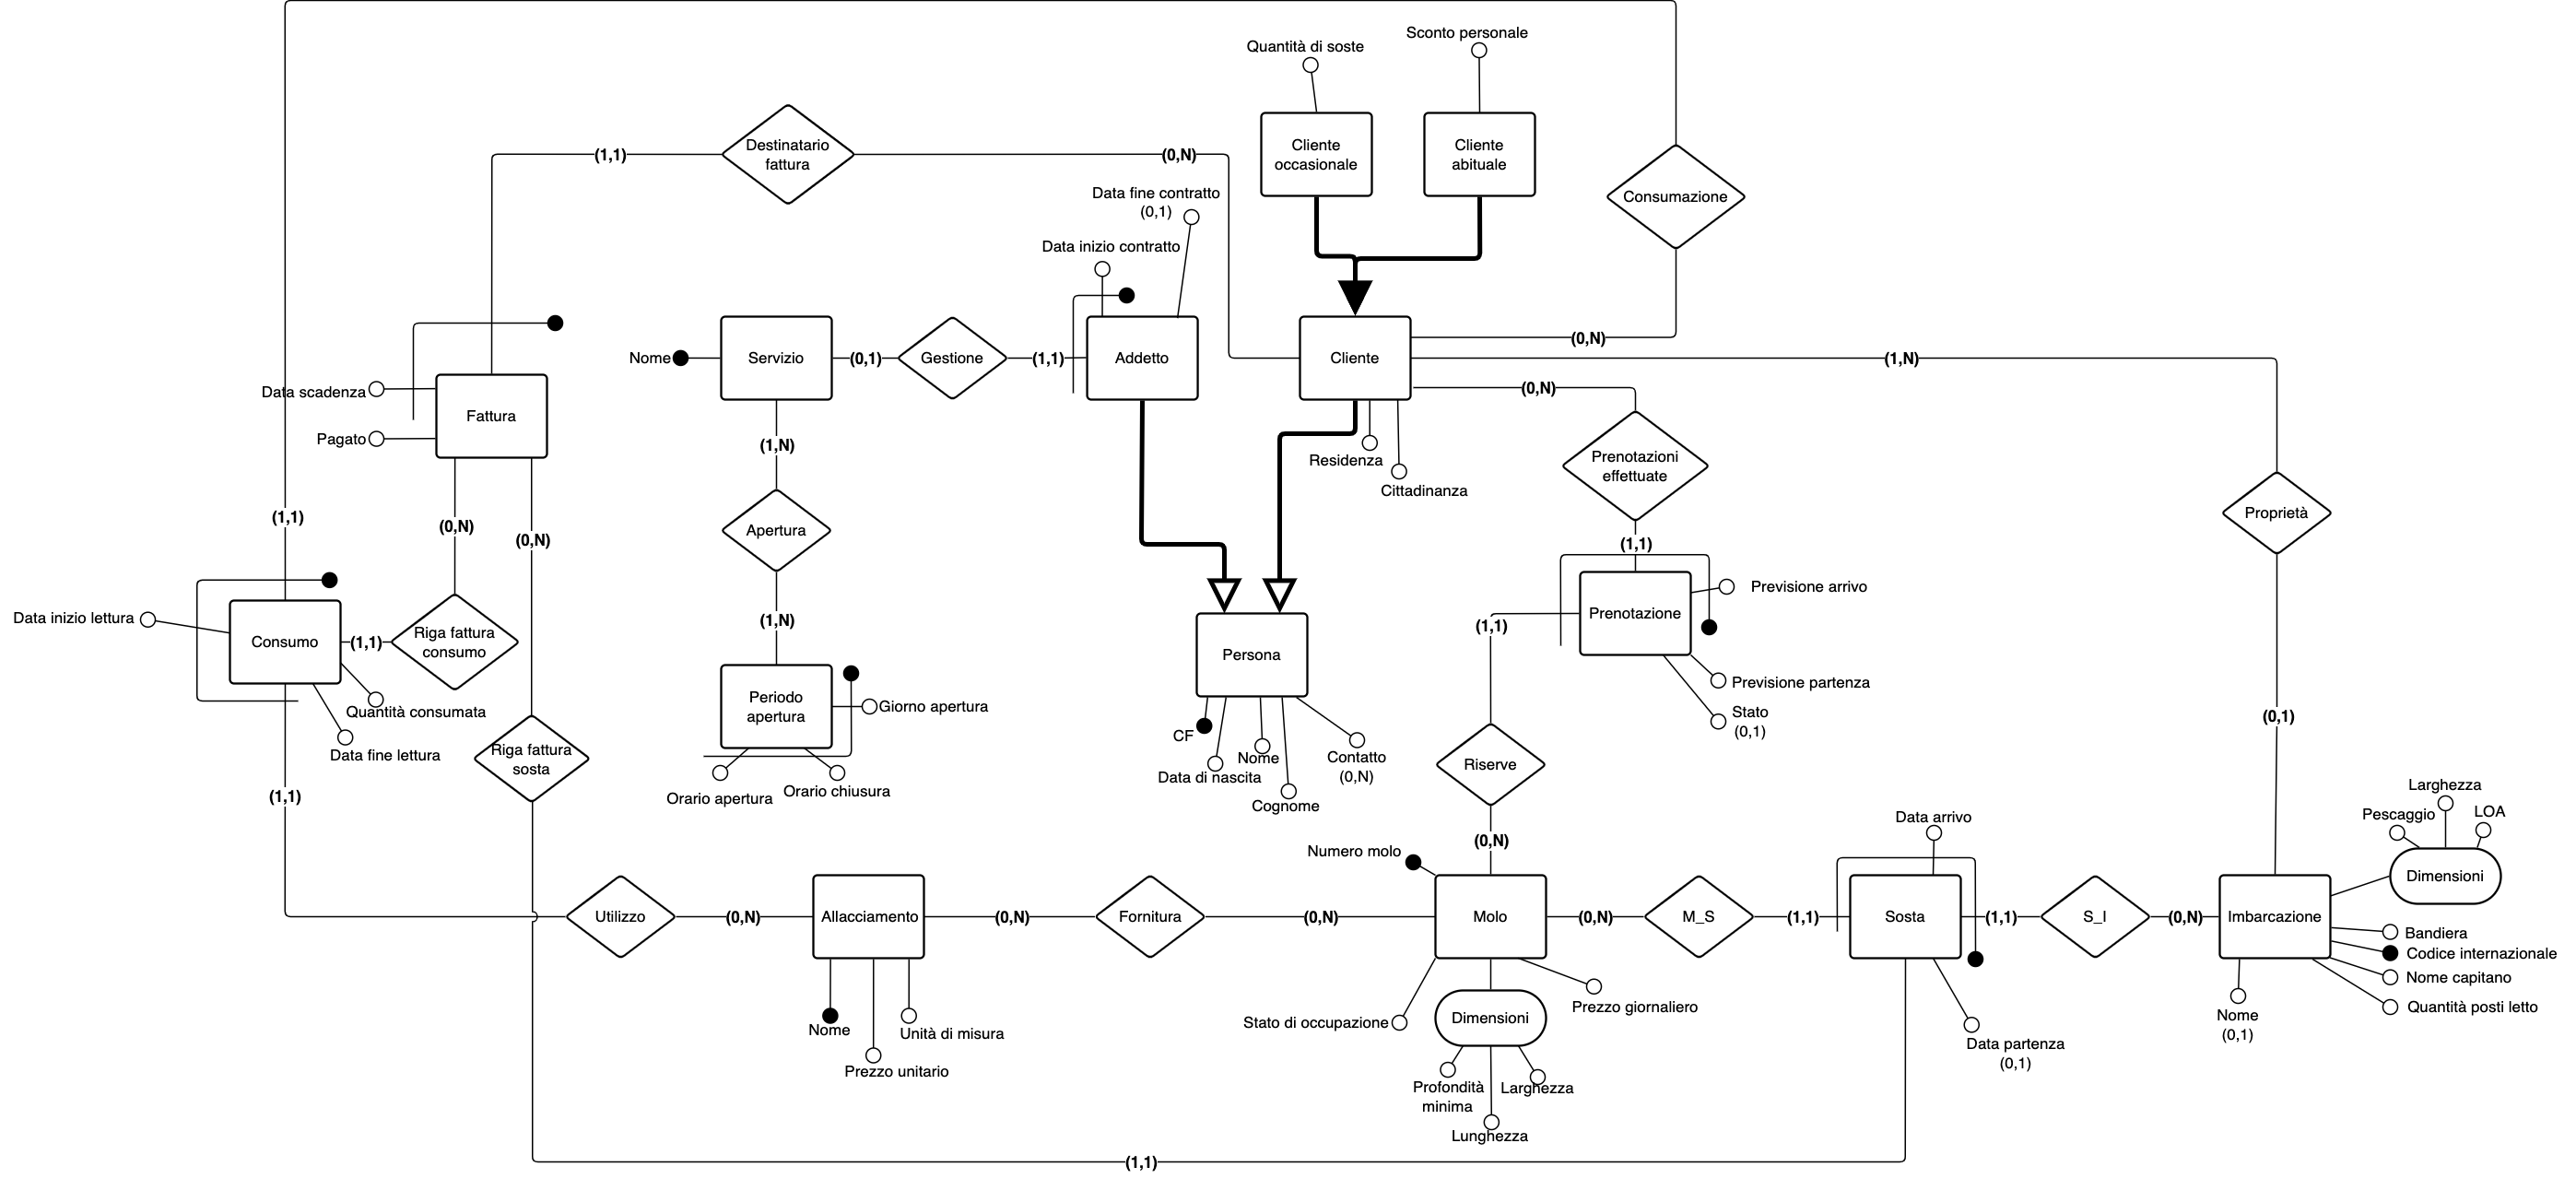
\includegraphics[width=\textwidth]{img/erconcettuale.png}